\section{Kommunikation}
\label{sec:kommunikation}

Zum Betreiben von \textit{Silisloth} sind mehrere Computer involviert:

\begin{itemize}
    \item In \textit{Silisloth} integrierte Computer
        \begin{itemize}
            \item Raspberry Pi: Steuerung, Bildverarbeitung, Ultraschallsensoren, Mikroendschalter
            \item Arduino: Steuerung von Schrittmotor, Getriebemotor, Luftpumpen und Ventil
        \end{itemize}
    \item Externe Computer
        \begin{itemize}
            \item Laptop: Aufstarten der Steuerungssoftware, Betrachten und Auswerten der Logdateien
            \item Smartphone: Erteilung des Startsignals, Überwachung der Lastkoordinaten
        \end{itemize}
\end{itemize}

Diese vier Computer müssen miteinander kommunizieren. \imgrefplain{fig:rechennetzwerk} zeigt, wie sie miteinander verbunden sind und welche Protokolle dabei zum Einsatz kommen.

\begin{figure}[H]
    \centering
    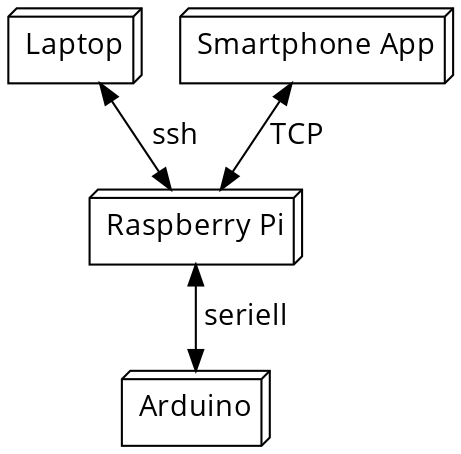
\includegraphics[width=0.5\textwidth]{graphs/rechennetzwerk.png}
    \caption{Die Verbindungen zwischen den vier involvierten Computern}
    \label{fig:rechennetzwerk}
\end{figure}

Das Sequenzdiagramm am Ende des Abschnitts (\imgref{fig:kommunikation}) bietet einen abschliessenden Überblick bezüglich der Kommunikation zwischen den vier involvierten Computern beim Absolvieren der Wettbewerbsaufgabe.

\subsection{Laptop -- Raspi}

Der Laptop verbindet sich per \texttt{ssh} mit dem Raspi. Da die IP-Adresse des Raspi nicht konstant ist, erfolgt die Verbindungsaufnahme über ein Skript, das in  der Dokumentation zu PREN 1 \cite[S. 34]{pren1} beschrieben ist. Ein Raspi ist seit Mitte Semester fix auf dem Prototypen verbaut. Damit auch zu Hause Tests mit einzelnen Komponenten durchgeführt werden konnten, kam ein weiterer Raspi zum Einsatz. Dieser hat eine andere MAC-Adresse als derjenige, der auf dem Prototypen verbaut ist. Das \textit{raspi-ssh}-Skript wurde für das komfortable Auffinden des richtigen Raspis im Netzwerk deshalb parametrisiert.

\subsection{Raspi -- Arduino}
\label{sec:raspi-arduino}

Die Kommunikation zwischen Raspi und Arduino erfolgt per serieller Verbindung über ein USB-Kabel. Die Kommunikation geht in beide Richtungen. Die Befehle wurden so kurz wie möglich gehalten und bestehen nur aus einem möglichst selbstsprechenden Zeichen (\tblref{tbl:raspi-arduino}). Eine Ausnahme bildet der «Stop»-Befehl, der zusätzlich einen ganzzahligen Parameter erwartet. Das Ende dieses Parameters wird mit einem Semikolon markiert.

Auf dem Arduino läuft ein Kommunikationstask, der Befehle parallel zur eigentlichen Steuerungslogik empfangen kann. Der Raspi wartet hingegen blockierend auf die Kommunikation vom Arduino, da es in den betreffenden Phasen auf dem Raspi nichts zu tun gibt. Threads würden an dieser Stelle nichts bringen und nur unnötig die Komplexität erhöhen.

\begin{table}
    \small
    \begin{tabularx}{\textwidth}{l|X|l}
        \textsc{Syntax} & \textsc{Semantik} & \textsc{Sender → Empfänger} \\
        \hline
        \texttt{G} & «Go» für losfahren bzw. weiterfahren & Raspi → Arduino \\
        \texttt{Sxxx;} & «Stop» mit \texttt{xxx} als vertikale Distanz in $mm$ zur Last & Raspi → Arduino \\
        \texttt{D} & «Decelerate» für verlangsamen & Raspi → Arduino \\
        \texttt{L} & «Load ready» für Last bereit (aufgenommen/abgesetzt) & Arduino → Raspi \\
        \texttt{H} & «Halt» für anhalten (und beenden) & Raspi → Arduino
    \end{tabularx}
    \caption{Die Befehle für das Kommunikationsprotokoll zwischen Raspi und Arduino}
    \label{tbl:raspi-arduino}
\end{table}

Zu Beginn des Projekts wurden die Befehle nicht in einzelne Zeichen sondern in ganzen Wörtern kodiert. Das hat den Vorteil, dass ganze Wörter selbstsprechend sind und das Protokoll so selbsterklärend wird. Die Übertragung dieser Strings wurde beidseitig mit gepuffertem I/O umgesetzt. Dies führte jedoch zu starken Verzögerungen bei der Kommunikation. Deshalb wurde auf ein primitiveres Protokoll gewechselt, bei dem nur einzelne Bytes geschrieben und gelesen werden müssen. Das Parsen eines ganzzahligen Parameters erforderte jedoch etwas zusätzliche Programmlogik.\footnote{Die Höhe wird bewusst in Millimetern und nicht in Zentimetern angegeben, da das Auslesen einer Fliesskommazahl wesentlich schwieriger ist als das Auslesen einer Ganzzahl.}

\subsection{Smartphone-App -- Raspi}

Die Kommunikation zwischen Smartphone-App und Raspi erfolgt über eine TCP-Verbindung. Der Raspi übernimmt dabei die Rolle des Servers. Das Steuerungsprogramm auf dem Raspi wird aufgestartet und wartet auf eine Verbindung. Wird auf der Smartphone-App die Schaltfläche \textit{Start} betätigt, wird die Verbindung mit dem Server (Raspi) aufgenommen. Dies gilt sogleich als Startsignal.

Ist die Last aufgenommen, werden die x- und z-Koordinaten an die Smartphone-App übertragen. Die beiden Parameter werden in eine Zeichenkette der Form \texttt{x=XXX;z=ZZZ\textbackslash{r}\textbackslash{n}} übertragen, wobei \texttt{XXX} und \texttt{ZZZ} für Distanzangaben in Millimetern stehen. Die Nachricht wird mit der Zeichenfolge \textit{carriage return} (\texttt{\textbackslash{r}}), \texttt{new line} (\texttt{\textbackslash{n}}) terminiert. Auf der Smartphone-App wird diese Zeichenkette geparst, und die Koordinaten werden in den entsprechenden Textfeldern angezeigt.

\begin{figure}
    \centering
    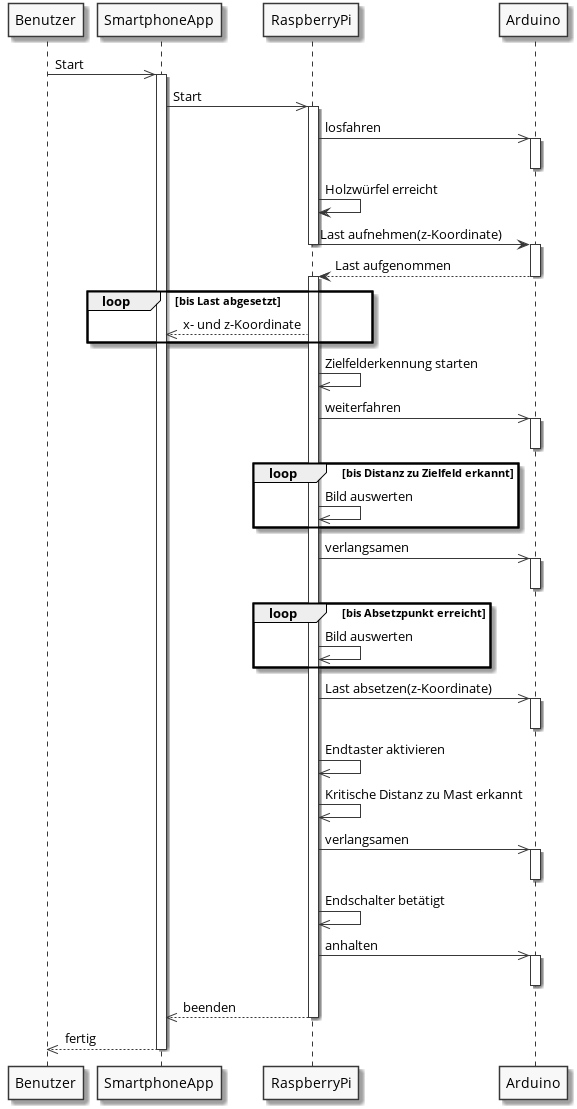
\includegraphics[height=\textheight]{graphs/sequenzdiagramm.png}
    \caption{Die Kommunikation zwischen Benutzer, Smartphone, Raspi und Arduino}
    \label{fig:kommunikation}
\end{figure}
